
\chapter*{PREFACE}
\addcontentsline{toc}{chapter}{PREFACE}

The documentation of WOFOST version 6.0 is based on the work of the following
researchers of DLO-CABO, Theoretical Production Ecology and SC-DLO: C.T. de
Wit, C.A. van Diepen, C.J.T. Spitters, F.W.T. Penning de Vries, H. van Keulen, N.G.
Seligman, J. Goudriaan, D.W.G. van Kraalingen, C. Rappoldt, H.F.M. ten Berge, R.
Rabbinge, H.H. van Laar, S.A. Ward, D.M. Jansen, A. Bakema and J. Wolf.
\newpage

\chapter*{INTRODUCTION}
\addcontentsline{toc}{chapter}{INTRODUCTION}

The Directorate General for Agriculture of the EC requires timely forecasting of
agricultural production to support the Common Agricultural Policy (CAP). 
Integration of Community statistics has until now been performed by the Statistical Office of
the European Community (O.S.C.E. or Eurostat) in Luxembourg. Prediction of yields
by Eurostat is based on statistical methods, using historical data. Time trends and
weather indicators are also taken into account. The Institute for Remote Sensing
Applications (IRSA) of the Joint Research Centre (JRC) of the EC, located in Ispra,
Italy, is in charge of a program to improve agricultural yield forecasts. This program
is known as the Agriculture Project or MARS project. Within the framework of this
project, an Advanced System of Information on Agriculture is being developed. Three
methods are being investigated by JRC: conventional surveys, remote sensing and
agro-meteorological modelling.

At the request of the JRC, the DLO Winand Staring Centre (SC-DLO) in co-operation with the 
DLO Centre for Agrobiological Research (CABO-DLO) in
Wageningen, The Netherlands, has executed the project:"Development, validation of
crop specific agrometeorological simulation models". The objective, as described in
the contract was "to develop, validate and test new or already existing agro-meteorological simulation models for 10-day routine quantitative forecasting of national and
NUTS-1 yields  and for 10-day areawise (regional), but qualitative monitoring of
agricultural season conditions over the whole of the EC and for each of the following
crops: wheat (spring and winter; hard and soft), barley (spring an winter), oats, maize
(grain), rice, potato, sugar beet, pulses (human consumption), soybean, oilseed rape,
sunflower, tobacco and cotton."  The Winand Staring Centre (SC-DLO) and the DLO
Centre for Agrobiological Research (CABO-DLO) have adapted the already existing
WOFOST crop growth model for this purpose.

WOFOST is the acronym for WOrld FOod STudies. It is the name of a model for
simulating the growth of crops. It was developed by the Centre for World Food
Studies in Wageningen, The Netherlands, in cooperation with the Agricultural
University and the Centre for Agrobiological Research (CABO). The version of the
model described here is called WOFOST 6.0. Earlier versions of the WOFOST
model are described by C. van Diepen et al. (1988 and 1989). The model describes
the growth and production of annual crops in physical terms determined by crop
species, soil type, hydrologic conditions and weather during the growing season. In
principle the model is applicable anywhere where crops are produced although the
model has been developed primarily for agriculture in the tropics.

The WOFOST simulation model is a tool for analysing the growth and production of
crops under a wide range of weather and soil conditions. Such analysis is important,
first to assess to what extend the crop production is limited by factors of light,
moisture and macro-nutrients, and second, to estimate what improvements are
possible.

\chapter{CROP GROWTH} 

\section{Systems, models and simulation}

\subsection{Definitions}
System analysis and simulation has been used by engineers for more than 30 years.
Their successes inspired biologist and agronomist to apply similar techniques in their
disciplines. The approach is characterized by the terms: systems, models and 
simulation (de Wit, 1982). A system is a limited part of reality that contains interrelated
elements. A model is a simplified representation of a system and simulation is may be
defined as the art of building mathematical models and the study of their properties
in reference to those of the system.

Although any model should have definite goals, be lucid and achieve its objective, in
practice it seems that goals are too often described in such broad terms that sufficient
lucidity  is reached only for the initiated, and that the models achieve less than
expected by the biologist. For these reasons the word 'art' rather than science is used
in the definition (de Wit, 1982).

\subsection{Descriptive models}
As described by Penning de Vries et al. (1989), a crop model is a simple representation of a 
crop. It is used to study the crop growth and to compute growth responses
to the environment. Crop models in common use can be distinguished as descriptive
and explanatory models. A descriptive model defines the behavior of a system in a
simple manner. The model reflects little or none of the mechanisms that are the
cause of the behavior. Creating and using this type of model is relatively straightforward. 
They often consists of one ore more mathematical equations. Those equations
have a limited validity. They can only be used for a specific cultivar and or soil type.
Descriptive models are therefore of value only for situations where interpolation
between observations is sought and there is no attempt to quantify the processes
involved.

\subsection{Explanatory model}
An explanatory model consists of a quantitative description of the mechanisms and
processes that cause the behaviour of a system. These descriptions are explicit
statements of the scientific theory and hypotheses. To create an explanatory model,
the system is analyzed and its processes and mechanisms are quantified separately.
The model is built by integrating these descriptions for the entire system. An
explanatory crop growth model contains descriptions of distinct processes such as
photosynthesis, leaf area expansion and tiller induction. Crop growth is a consequence 
of these underlying processes.

If all the elements, composing the model are well understood it may not be necessary
to evaluate the model by comparing its results with those of the real system. 
Explanatory models in biology are so rudimentary, however, that proof of their usefulness is
necessary. Good agreement between predictions and observations is still more the
exception than the rule, and even when there is good agreement there is room for
doubt (Rabbinge \& de Wit, 1989). If there are discrepancies between the model and
the real system, the model may be adjusted by tuning variables to obtain better
agreement. The explanatory model can thus be degenerated to a descriptive model. It
might then be better to use statistically efficient models designed for this purpose,
such as multivariate regression models used by Thompson (1969), Pitter (1977) and
Bridge (1976).

The appropriate approach in explanatory modelling is heuristic, by way of gradual
improvement. If unacceptable discrepancies between model and system are observed,
it may be possible to judge which aspects are then to be studied experimentally on
the level of used for explanation. Explanatory models can thus be used to guide
research.

\subsection{Levels of crop production}
De Wit proposed a classification of systems growth-limiting factors (de Wit \&
Penning de Vries, 1982; Penning de Vries \& van Laar, 1982). Four levels of plant
production are distinguished. The crop production systems at any of these levels can
be considered as members of a broad class. In order of decreasing yield, these levels
are (Penning de Vries et al. 1989):

{\it Production level 1\/}\\
This is the potential production situation. The crop has ample water and nutrients.
Crop growth depends on the current state and wheater (temperature and radiation.
Dry matter production, in case of full canopy, amounts 150-350 kg ha$^{{\rm -1}}$d$^{{\rm -1}}$. This
production level will be reached in laboratory experiments, glasshouses and with
intensive farming systems.

{\it Production level 2\/}\\
The crop growth is limited by the availability of water during a part or the complete
growing season. This situation occurs in semi-arid regions when fertilizers are applied
or in other climates when light soils are intensively used.

{\it Production level 3\/}\\
The crop growth is limited by the availability of nitrogen for at least a part of the
growing season and by water availability or poor weather conditions for the remainder
of the growth period. This situation is quite common all over the world. It should be
noted that in the natural environment even nitrogen-efficient plant cannot always
absorb sufficient nitrogen.

{\it Production level 4\/}\\
The crop growth is limited by the availability of phosphorus and other mineral
nutrients for at least a part of the growing season. Dry matter production amounts
10-50 kg ha$^{{\rm -1}}$d$^{{\rm -1}}$ and the growing season often lasts less then hundred days. This
situation is quiet common in cases where the soil is heavily exploited and no fertilizers are used. 

\section{Application of crop growth models}
Crop growth simulation models can be applied in the domain of potential crop
production and production with a temporary water shortage but ample nutrients
(production levels 1 and 2). These domains include predicting short term yield,
extrapolating and interpolating crop performance over large regions and simplifying
and combining with other models to create links with other sciences (Penning de
Vries, 1989). Applying models can lead to more effective use of existing knowledge
for extension, agronomic and cropping systems research and breeding and to more
efficient experimentation. Whisler et al. (1986) presented an overview of crop models
and their application.

Crop yields can be predicted some time before harvest by using expected weather
data. This might be important for cash-crops, where trade and planning post harvest
activities start early.
Van Keulen \& Wolf (1986) have used a crop growth model to estimate yield levels of
various food crops on a regional scale where there were no or insufficient external
inputs to ensure potential growth.

\subsection{The WOFOST crop growth model}
The crop growth simulation model WOFOST version 6.0 can be used for the same
purpose as the preceding versions of WOFOST described by Wolf et al. and by
Rappoldt (1986): the assessment of agricultural production potentials and of the
constraining growth factors as influenced by environmental conditions, reclamation
measures and management. The model can be considered as a system approach for
analyzing the bio-physical aspects of the production of annual crops, grown in
monoculture. This version of WOFOST allows quantification of obtainable crop
yields for two well defined production situations. The first one is the potential
production situation, production level 1 and the second is the water limited situation,
production level 2.

\subsection{Processed described in WOFOST}
A Crop Growth Simulation model basically is a set of equations describing physical
processes. Sunlight is the driving force for crop growth. The intensity of radiation, the
interception of light and the efficiency of energy use in the plant are the main factors
which influence the photosynthesis. The environmental temperature plays also an
important role. It influences both the photosynthetic rate and growth rate. The
assimilates which are not used for the maintenance are partitioned over the roots,
stems, leaves and storage organs.Partitioning of the assimilates is dependent on the
development stage which on its turn is related to the temperature sum. Structural
biomass cannot be mobilized for either maintenance or growth processes elsewhere in
the plant.

Water shortage leads to stomatal closure and simultaneous reduction of assimilation
and transpiration. The ratio of the actual transpiration rate and the potential rate
provides the link between the carbon and the water balance. The extent to which the
potential photosynthesis is realized, depends on the availability of water.

A System Description provides information on these processes and how they are
described in the simulation model. Into more detail a system description will 
consider:
\begin{itemize}
\item Functionality
\item Processes
\item Data
\item Implementation
\end{itemize}

{\it 1. Functionality}\\
The System Description describes the functions to be performed by the program.
What should the program be able to do. 

{\it 2. Processes}\\
Functionalities can be translated to processes. One function can be described with
one or more processes. Processes described in a simulation model will have a
scientific basis.\\
These processes can be described using equations. These equations will be described
in a System Description, with their scientific background which explains the use of the
equations. 

{\it 3. Data}\\
A System Description describes the data needed as input to the equations as
described in the description of the processes. 

{\it 4. Implementation}\\
The processes have to be ordered in a rational way to simulate crop growth. The
description of the implementation of the processes is also part of the user manual.
This means a description of the subroutines in relation to the described processes and
a calling structure of these subroutines.  

This implies that a System description does not describe:
\begin{itemize}
\item the actual implementation of the equations in the model (code);
\item A model has to be implemented in a certain computer language which has its
own rules. These rules will not be described. In the source code of the model 
(files with the extension .FOR) the actual implementation of all the equtions
can be found.
\item the different formats in which input can be delivered to the model;\\
A lot of input parameters are needed for the model to run. Values for
meteorological parameters, crop parameters, soil parameters and model
parameters need to be specified to run the model. This is done with the help
of input files. An extensive description of the input files is provided in the user
manual of the model (Guiking, 1993). In the description of the different
processes input parameters will be pointed out by telling that these input
parameters are station, crop or soil specific.   
\item information on the different output files that can be generated;\\
Different types of output files can be created according to the whishes of the
user. An extensive description of the output files is provided in the user
manual of the model (Guiking, 1993).
\item the user interface. \\
WOFOST offers the possibility to make a interactive run specification. This is
also described in the user manual (Guiking, 1993).
\end{itemize}

\section{Functional description of WOFOST Version 6.0}

Crop growth is often described by an empirical model, consisting of a regression
equation (e.g. a logistic function). Sometimes, environmental variables, such as
radiation and rainfall, are incorporated in the regression. These models can generate
accurate yield predictions, especially when the regression parameters are estimated on
the basis of extensive sets of experimental data. The predictions are restricted to the
same environment on which the regression is based. These empirical, descriptive
models, however, give little insight into the causes of the observed variation in yields. 

WOFOST Version 6.0 is a mechanistic model that explains crop growth on the basis
of the underlying processes, such as photosynthesis and respiration, and how these
processes are influenced by environmental conditions. The predictive ability of
mechanistic models does not always live up to expectation. It should be realized,
however, that each parameter estimate and process formulation has its own inaccuracy, 
and that these errors accumulate in the prediction of final yield. However, yield
prediction is a secondary aim of these models. Their primary aim is to improve
insight into the studied system by integrating the present knowledge quantitatively in
terms of a simulation model. By studying the behavior of the model, better insight
into the real system is gained.

Crop growth can be simulated for one crop for a number of growth seasons. Only
one growth season can be simulated for one calendar year.  The model explains crop
growth on the basis of the underlying processes, such as photosynthesis and respiration, 
and how these processes are influenced by environmental conditions.
Dry matter accumulation of a crop can thus be calculated as a function of irradiation,
temperature and crop characteristics.

The crop growth simulation model must keep track of the soil moisture potential to
determine when and to what degree a crop is exposed to water stress. This can be
done with the aid of a water balance, which compares for a given period of time,
incoming water in the rooted surface soil with outgoing water and quantifies the
difference between the two as a change in the amount of soil moisture stored.
Meteorological data (rain, wind speed, global radiation, sunshine duration, etc.) are
needed as input for the soil water balance. These data are often measured on a daily
basis. This is the reason why the time set for simulation is set to one day.

\begin{figure}[htbp]
% figure 1.1
\centering
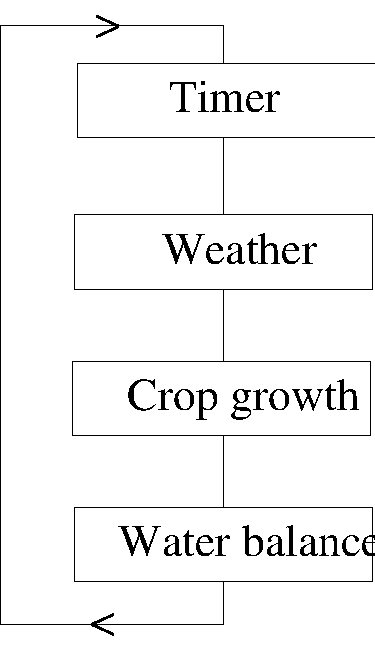
\includegraphics[width=70mm]{\FigDir/DAGLOOP.pdf}
\caption{Daily calculations}
\label{fig:dayloop}
% \begin{center}\InputPS{file=\FigDir/DAGLOOP.eps,width=7.04cm} \end{center}
\end{figure}

\begin{figure}[htbp]
% figure 1.2
\centering
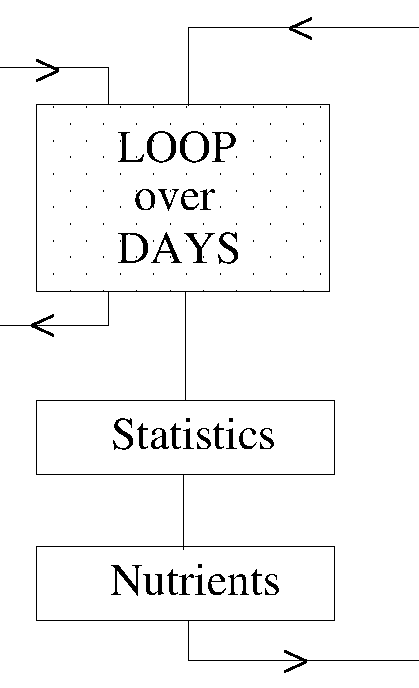
\includegraphics[width=70mm]{\FigDir/JAARLOOP.pdf}
\caption{Yearly calculations}
\label{fig:yearloop}
% \begin{center}\InputPS{file=\FigDir/JAARLOOP.eps,width=7.04cm} \end{center}
\end{figure}

The influence of nutrients (nitrogen, phosphate and potassium) on the yield and the
yield statistics are calculated on a yearly basis. 
Figure \ref{fig:dayloop} presents this loop over days for one growth season, 
whereas figure \ref{fig:yearloop} depicts the loop over years for one simulation run.
Another important feature of the crop growth simulation model is the comparison of
the potential production with the water limited production. The potential production
assumes that the soil moisture content is always at field capacity.

\begin{figure}[htbp]
\centering
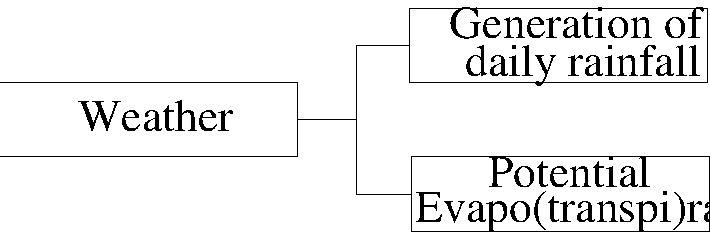
\includegraphics[width=77mm]{\FigDir/WEERLOOP.pdf}
% \begin{center}\InputPS{file=\FigDir/WEERLOOP.eps,width=7.73cm} \end{center}
\end{figure}

\begin{figure}[htbp]
\centering
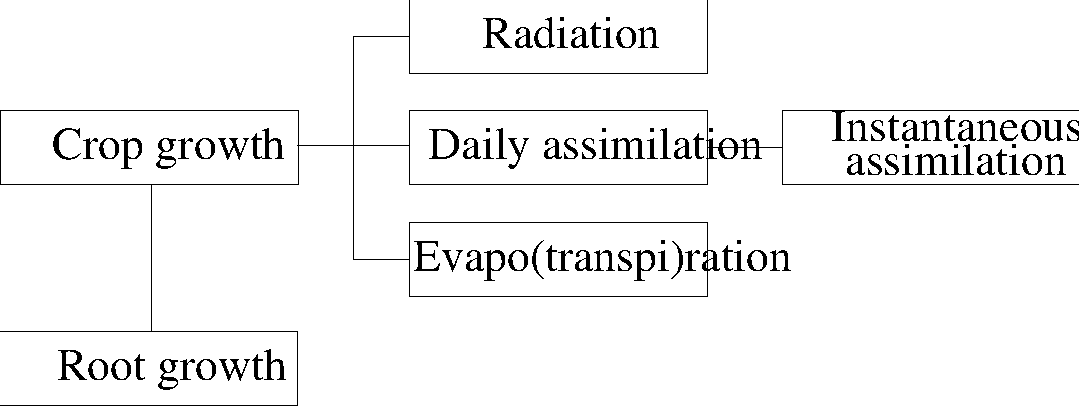
\includegraphics[width=93mm]{\FigDir/CROPLOOP.pdf}
% \begin{center}\InputPS{file=\FigDir/CROPLOOP.eps,width=9.29cm} \end{center}
\end{figure}

\begin{figure}[htbp]
\centering
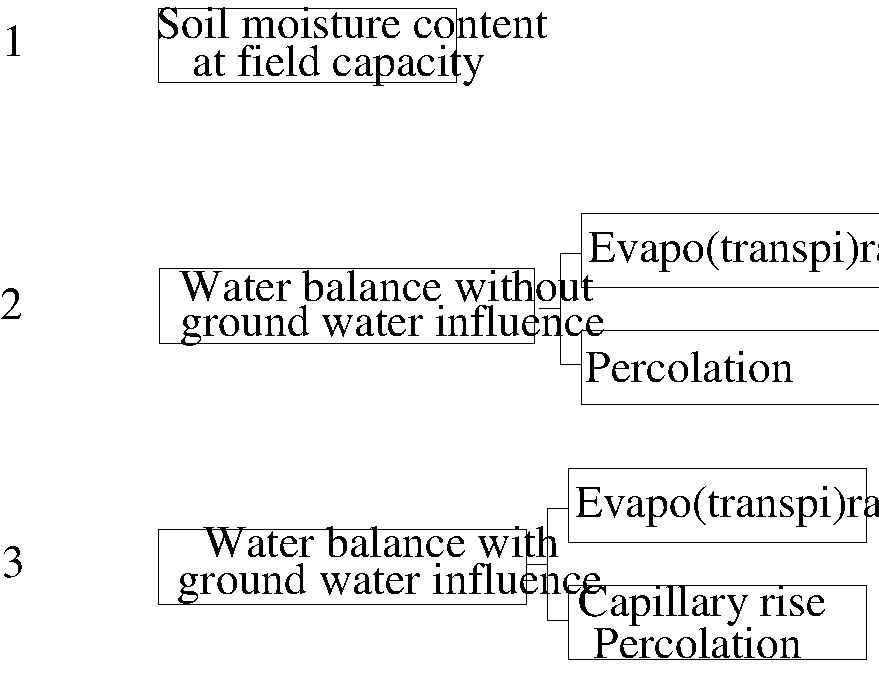
\includegraphics[width=93mm]{\FigDir/SOILLOOP.pdf}
% \begin{center}\InputPS{file=\FigDir/SOILLOOP.eps,width=9.29cm} \end{center}
\end{figure}

The model can be used to simulate production and water use in order to survey
and evaluate new sites, crops or cultivars, husbandry and management techniques 
before embarking on a large
program. The model can also establish the impact of year-to-year weather variability
on the crop much faster than with more conventional methods. 

This manual covers the processes of crop growth and water movement as they are
implemented in WOFOST Version 6.0. 
The next chapter contains an description of the implementation of the model. It
describes the programming environment, the structure of the model with its different
sub routines and functions, and the libraries used.
Chapter 3 discusses the calculation and conversion of meteorological data like:
calculation of potential evapo(trans)piration, calculation of day length and solar
elevation and deriving daily rainfall data from long term monthly rainfall data.
Chapter 4 discusses how the most important crop growth processes are simulated
like: daily assimilation, maintenance respiration, growth respiration, partitioning of
assimilates, senescence and death. Chapter 5 discusses the soil water balance
calculations. These calculations keep track of the water in the soil. The soil moisture
content can be calculated from this. 

van Diepen, C.A., Rappoldt, C., Wolf, J., van Keulen, H. 1988. {\it Crop growth simulation model}

{\it WOFOST version 4.1, documentation}. SOW-88-01. Centre for World
Food Studies, Wageningen, The Netherlands.

van Diepen, C.A., Wolf, J., van Keulen, H., Rappoldt C.,. 1989. {\it WOFOST: a simulation 
model of crop production.} Soil use and management, Volume 5, Number 1, March.
